\subsection{STEREOGRAPHIC PROJECTION}

Consider the point \(e_{n}=(0,\ldots,0,1)\) of \(S_{n-1}\) , and the hyperplane H with equation \(x_{n}=0\) , orthogonal to the vector \(e_{n}\) . To every point \(x=(x_{i})\) of \(S_{n-1}\) , other than \(e_{n}\) , let us make correspond the point y where the line through \(e_{n}\) and x meets the hyperplane H (Fig. 3). It is easily verified that we have

\[
\mathbf {y} = \frac {1}{1 - x _ {n}} (\mathbf {x} - x _ {n} \mathbf {e} _ {n})
\]

and

\[
\boldsymbol {x} = \frac {\left| \left| \boldsymbol {y} \right| \right| ^ {2} - 1}{\left| \left| \boldsymbol {y} \right| \right| ^ {2} + 1} \boldsymbol {e} _ {n} + \frac {2}{\left| \left| \boldsymbol {y} \right| \right| ^ {2} + 1} \boldsymbol {y}.
\]

\pandocbounded{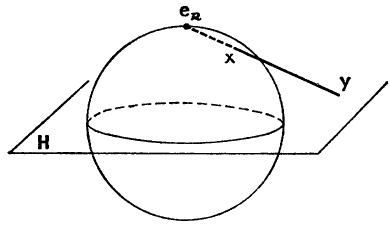
\includegraphics[keepaspectratio]{images/part001_990d2877.jpg}}\\
Figure 3.

If we denote by A the complement of \(\{e_{n}\}\) in \(S_{n-1}\) , these formulas show that we have thus defined a homeomorphism of A onto the hyperplane H. This homeomorphism is called the stereographic projection of A onto H, or (by abuse of language) the stereographic projection of \(S_{n-1}\) onto H; \(e_{n}\) is the vertex of the projection, H the hyperplane of projection. More generally, if \(H'\) is any hyperplane passing through o (a diametral hyperplane of \(B_{n}\) ) and if a is one of the points of intersection of \(S_{n-1}\) and the line orthogonal to \(H'\) passing through o, we can define in the same way the stereographic projection with vertex a onto the hyperplane of projection \(H'\) ; in any case this projection can be brought back to the preceding one by an orthogonal transformation which transforms \(H'\) into H and a into \(e_{n}\) .

PROPOSITION 4. If \(n > 1\) , the Euclidean sphere \(S_{n-1}\) is homeomorphic to the space \(\mathbf{R}^{n-1}\) made compact by adjoining a ``point at infinity'' (Chapter I, § 9, no. 8, Theorem 4).

For the stereographic projection defines a homeomorphism of the complement of a point in \(S_{n-1}\) onto a hyperplane of \(R^{n}\) , which is homeomorphic to \(R^{n-1}\) .

COROLLARY 1. The sphere \(S_{n}\) is homeomorphic to the quotient space of the ball \(B_{n}\) obtained by identifying all the points of the sphere \(S_{n-1}\) .

The ball \(B_{n}\) is a regular space (Chapter I, § 8, no. 4); hence the quotient space F of \(B_{n}\) obtained by identifying all the points of \(S_{n-1}\) is Hausdorff (Chapter I, § 8, no. 6, Proposition 15). Since \(B_{n}\) is compact, so is F, and F is therefore homeomorphic to an open ball of n dimensions made compact by adjoining a point at infinity, by Alexandroff's theorem (Chapter I, § 9, no. 8, Theorem 4). The result therefore follows from Propositions 2 and 4.

COROLLARY 2. The circle \(\mathbf{S}_1\) is homeomorphic to the torus \(\mathbf{T}\) .

In Chapter VIII, § 2, no. 1, we shall obtain this result again as a consequence of a more precise theorem.

PROPOSITION 5. If \(n > 1\) , the Euclidean sphere \(\mathbf{S}_{n-1}\) is connected and locally connected, and every point of it has an open neighbourhood homeomorphic to \(\mathbf{R}^{n-1}\) .

The complement of a point in \(S_{n-1}\) is a connected dense set, and therefore (Chapter I, § 11, no. 1, Proposition 1) \(S_{n-1}\) is connected. To see that every point has a neighbourhood homeomorphic to \(R^{n-1}\) , we have only to project stereographically from a vertex other than the given point.

From this proposition and from Proposition 3 of no. 3 it follows that \(\mathbf{R}_n^*\) , being the product of two connected spaces, is connected (Chapter I, § 11, no. 4, Proposition 8; cf.~§ 1, Exercise 10).

The intersection of \(S_{n-1}\) and a closed (resp. open) half-space determined by a diametral hyperplane of \(B_{n}\) is called a closed (resp. open) hemisphere of \(S_{n-1}\) . By stereographic projection onto the diametral hyperplane, the closed (resp. open) hemisphere which does not contain the vertex of projection is mapped onto a closed (resp. open) ball of n - 1 dimensions, to which it is therefore homeomorphic.

If n = 2, we say ``semicircle'' instead of ``hemisphere''.

